\documentclass[conference]{IEEEtran}
%\usepackage{cite}
\usepackage[pdftex]{graphicx}
\usepackage[cmex10]{amsmath}
\interdisplaylinepenalty=2500
\usepackage{algorithmic}
\usepackage{array}
\usepackage{mdwmath}
\usepackage{mdwtab}
\usepackage{eqparbox}
\usepackage[caption=false,font=footnotesize]{subfig}
\usepackage{fixltx2e}
%\usepackage{stfloats}
\usepackage{url}
\hyphenation{op-tical net-works semi-conduc-tor}

% additional packages and utility commands
\usepackage{color}

\newcommand{\TODO}{\textbf{\color{red}TODO}}

\begin{document}

\title{Lowering the Impact of Intrusion Detection\\
on Resources in Wireless Sensor Networks\\
using Code Generation Techniques}

\author{\IEEEauthorblockN{Christophe Van Ginneken, Jef Maerien, Christophe
Huygens, Danny Hughes, Wouter Joosen}%
\IEEEauthorblockA{iMinds - DistriNet - KULeuven\\
B-3001, Leuven, Belgium\\
Christophe.VanGinneken@student.kuleuven.be,\{firstname.lastname\}@cs.kuleuven.be}}

\maketitle

\begin{abstract}
\TODO
\end{abstract}

\section{Introduction}

\TODO

\subsection{Subsection Heading Here}

\TODO


\subsubsection{Subsubsection Heading Here}

\TODO

Subsubsection text here.

\begin{figure}[!t]
\centering
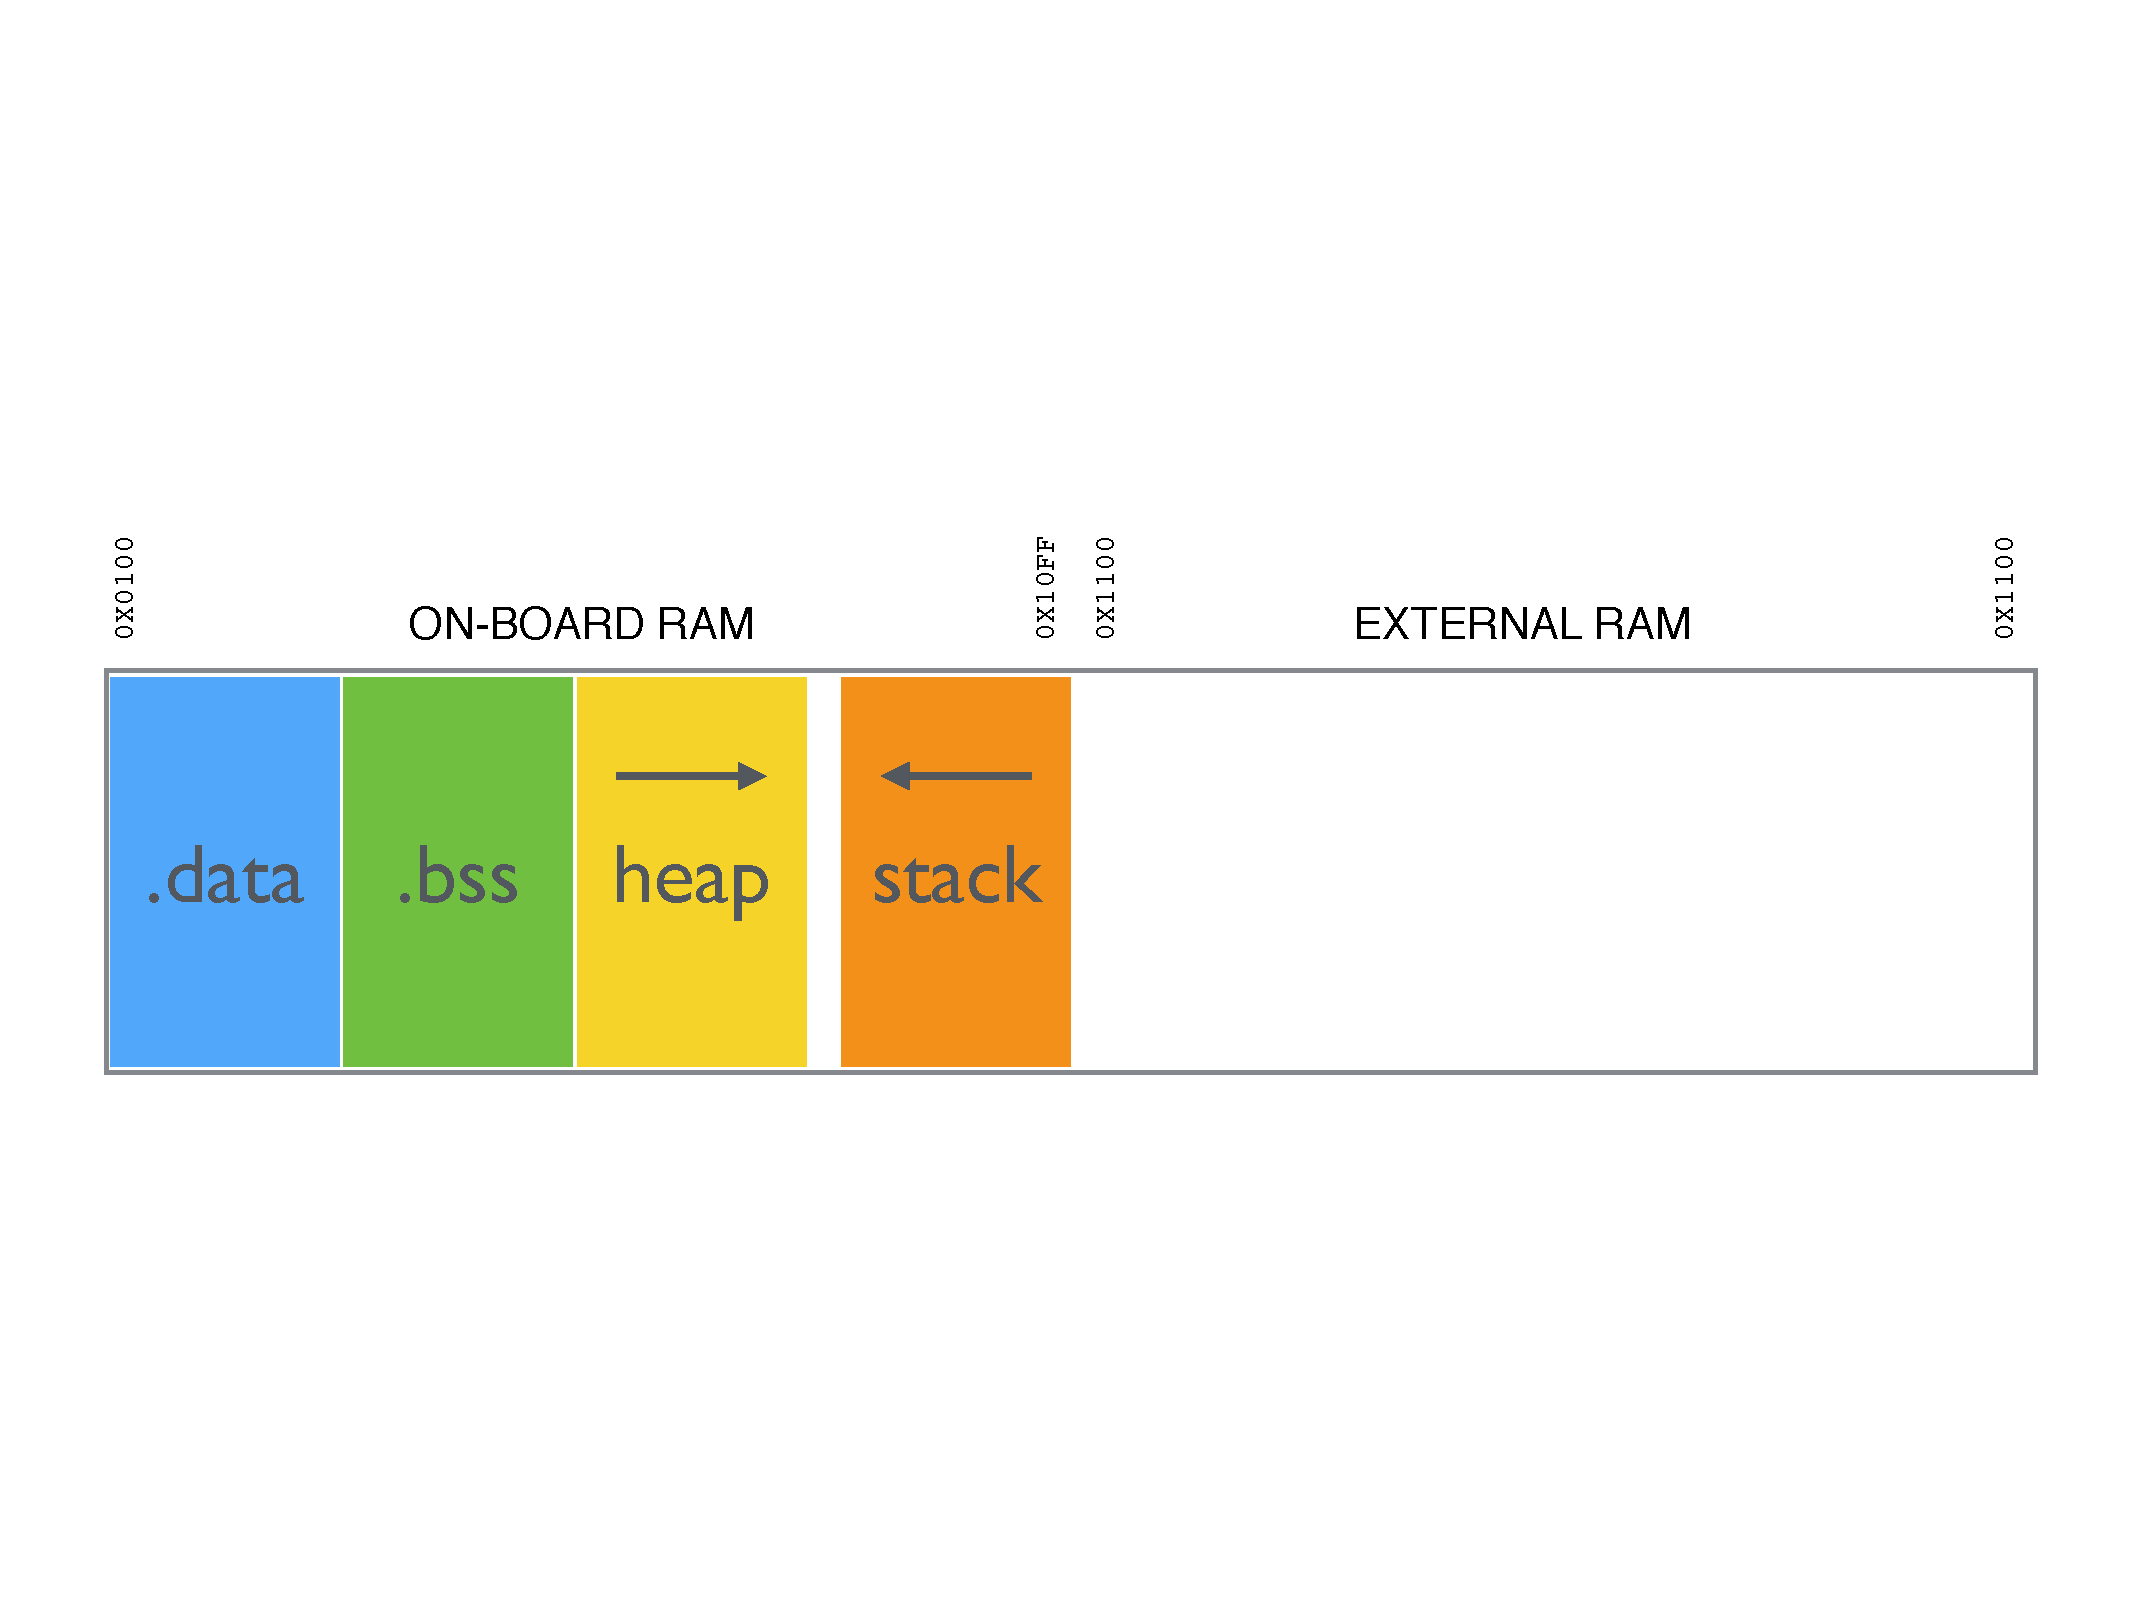
\includegraphics[width=2.5in]{resources/avr-ram-map.pdf}
\caption{Simulation Results}
\label{fig_sim1}
\end{figure}

\begin{figure*}[H]
\centering
\subfloat[]{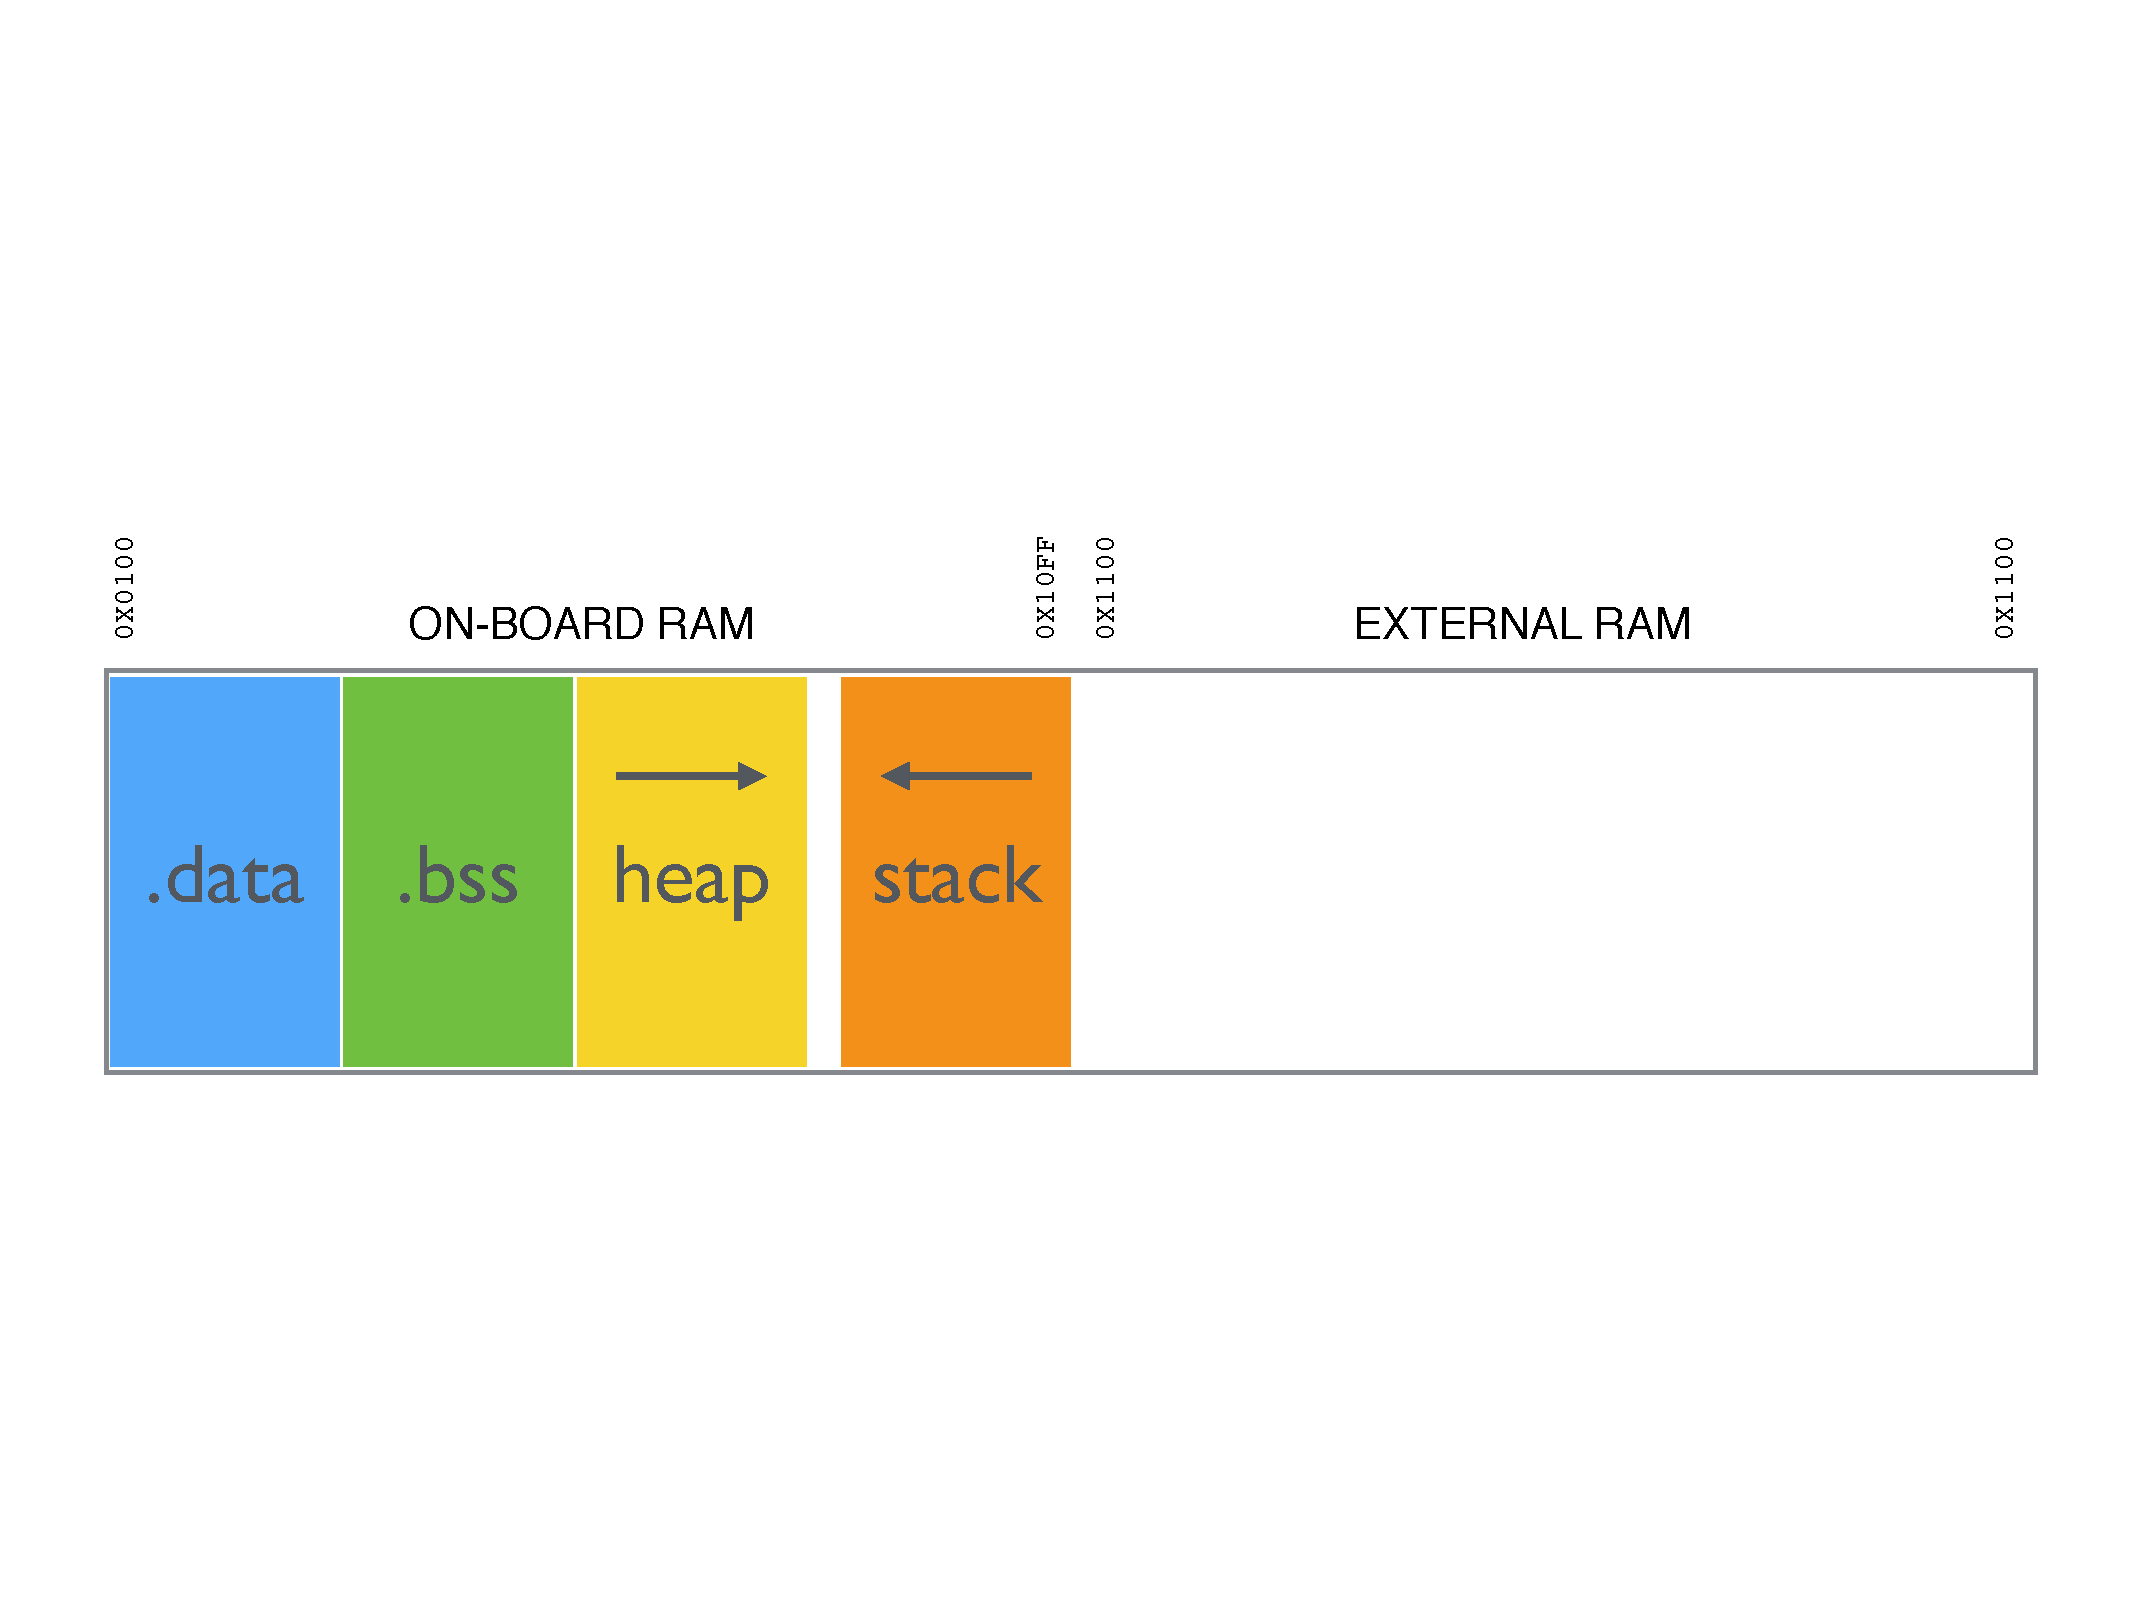
\includegraphics[width=2.5in]{resources/avr-ram-map.pdf}%
\label{fig_first_case}}
\hfil
\subfloat[]{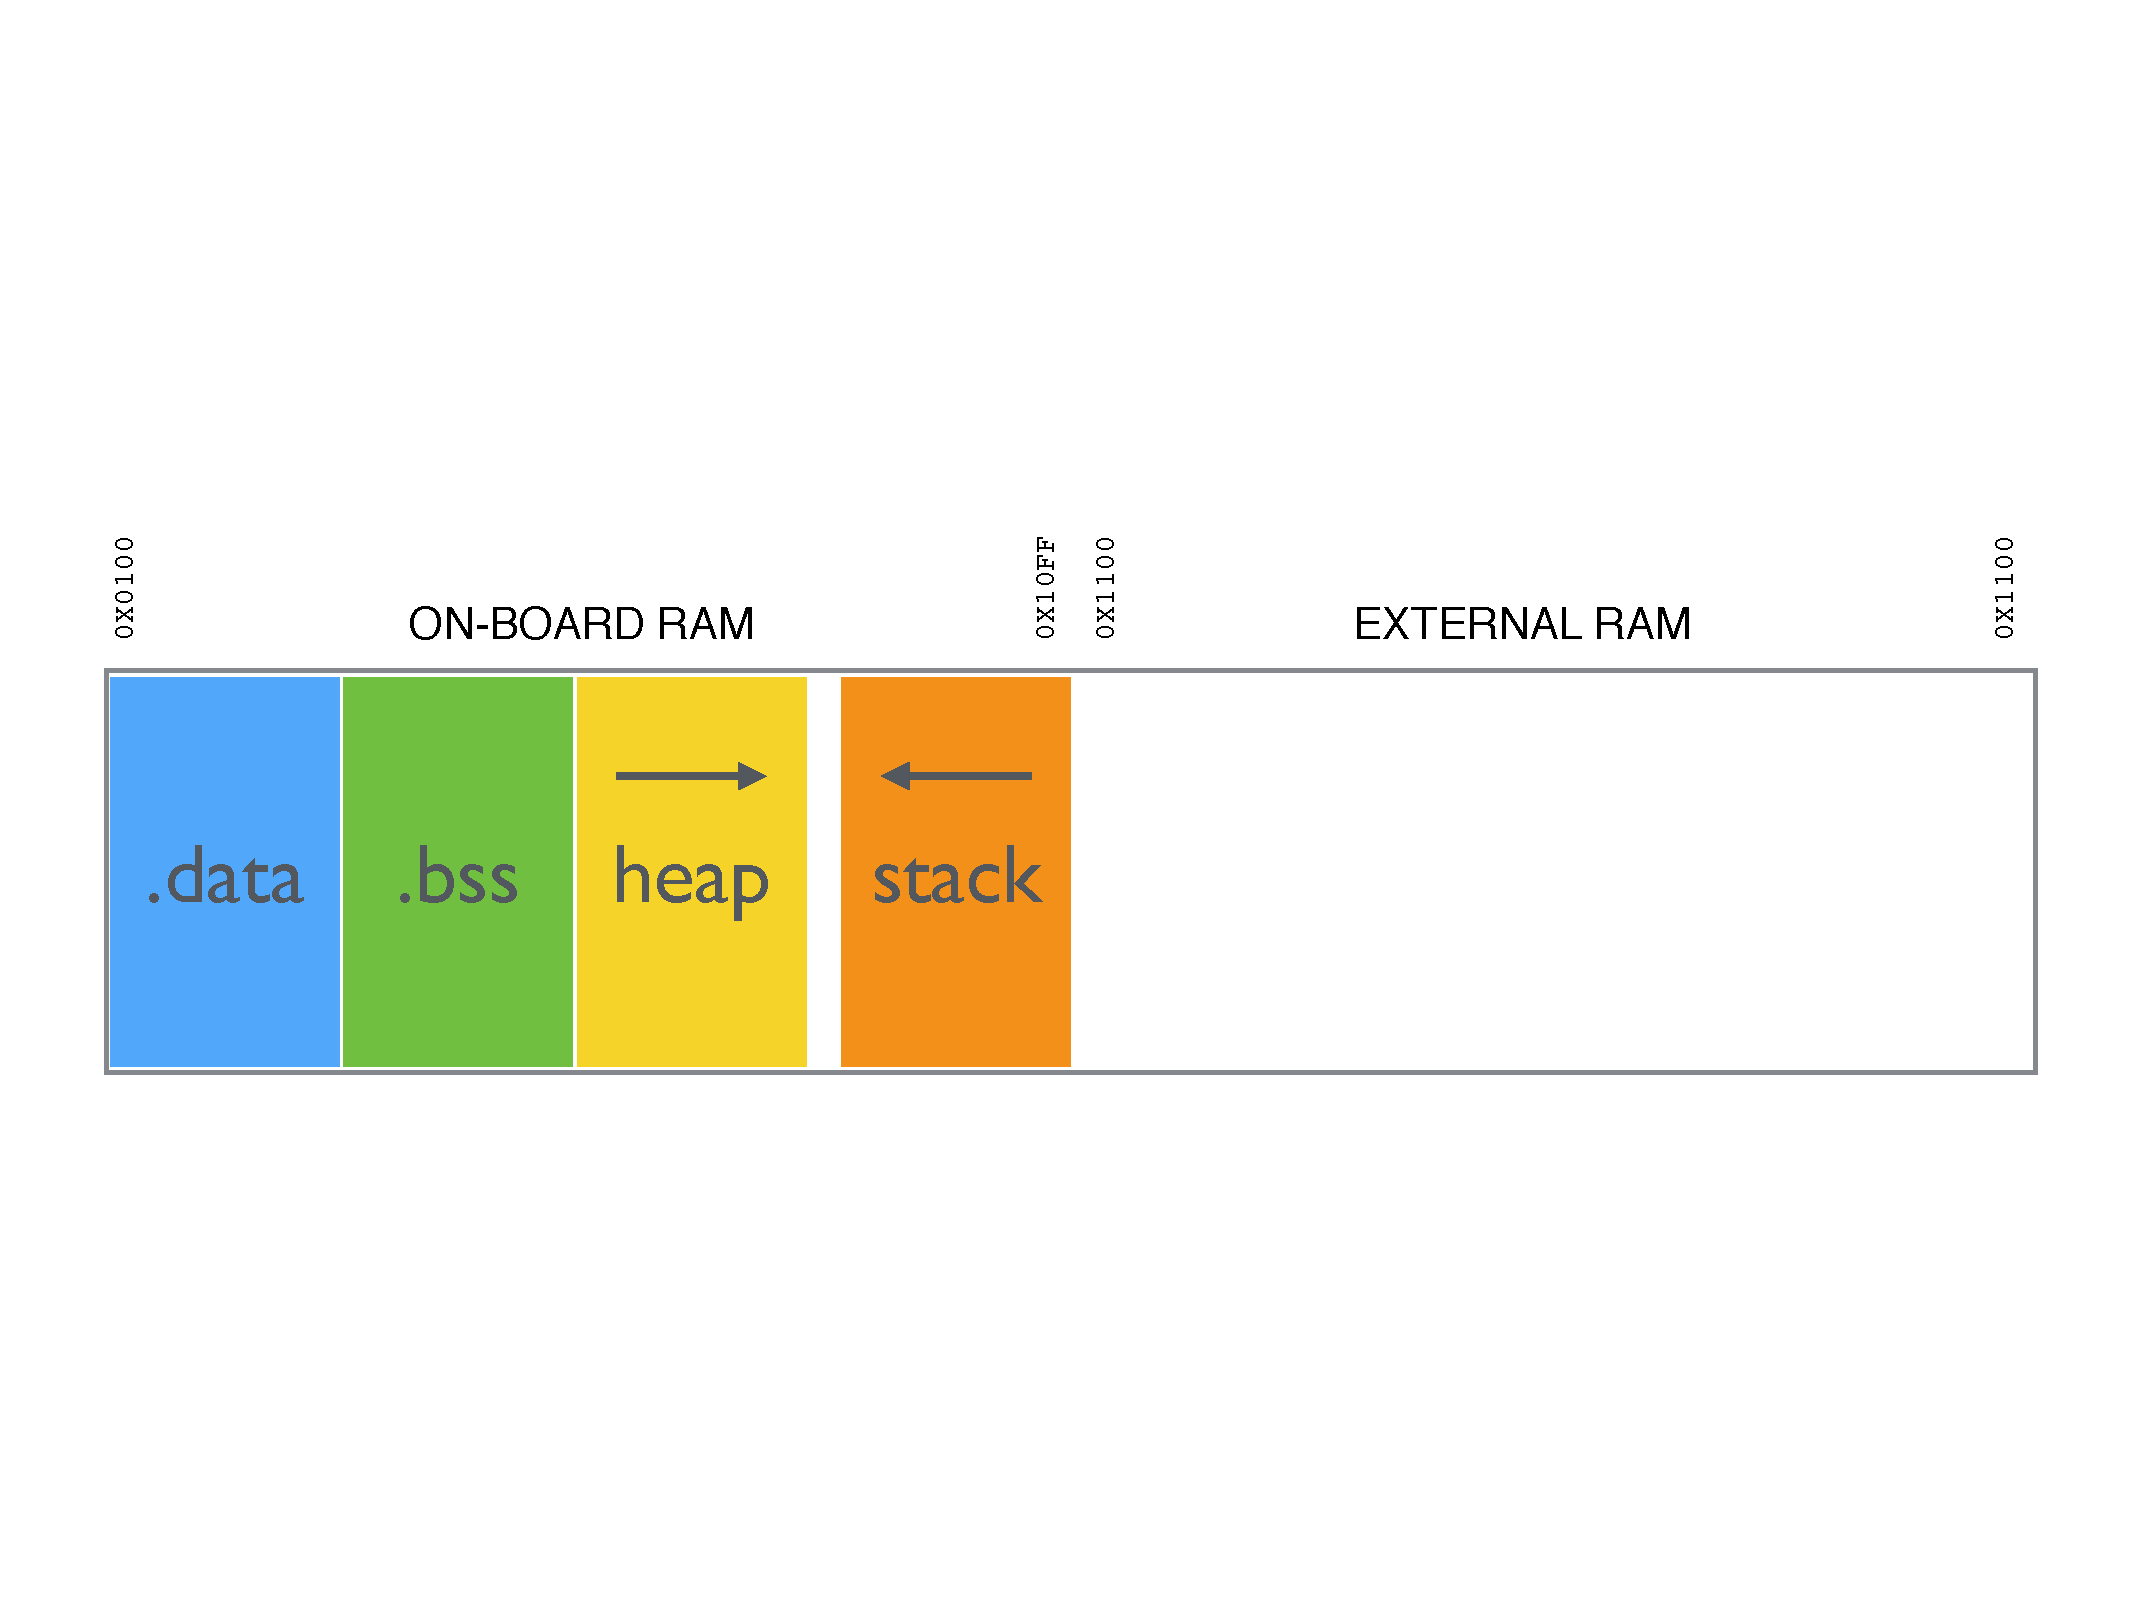
\includegraphics[width=2.5in]{resources/avr-ram-map.pdf}%
\label{fig_second_case}}
\caption{Simulation results: (a) Case I (b) Case II}
\label{fig_sim2}
\end{figure*}

\begin{table}[!t]
\renewcommand{\arraystretch}{1.3}
\caption{An Example of a Table}
\label{table_example}
\centering
\begin{tabular}{|c||c|}
\hline
One & Two\\
\hline
Three & Four\\
\hline
\end{tabular}
\end{table}

\section{Related Work}

With FAMOS\cite{maerien2012famos}, \dots

\TODO

\section{Problem Analysis}

\TODO

\section{Introducing the FOO Language}

\TODO

\section{Evaluation}

\TODO

\section{Conclusions and Further Work}

\TODO

% conference papers do not normally have an appendix

% use section* for acknowledgement
\section*{Acknowledgment}

The authors would like to thank... \TODO

% \IEEEtriggeratref{1}

\bibliographystyle{IEEEtran}
\bibliography{referenties}

\end{document}


